% Created 2022-03-18 Fri 11:58
% Intended LaTeX compiler: pdflatex
\documentclass[a4paper, 11pt]{article}
\usepackage[utf8]{inputenc}
\usepackage[T1]{fontenc}
\usepackage{graphicx}
\usepackage{longtable}
\usepackage{wrapfig}
\usepackage{rotating}
\usepackage[normalem]{ulem}
\usepackage{amsmath}
\usepackage{amssymb}
\usepackage{capt-of}
\usepackage{hyperref}
\usepackage[margin=1.25in]{geometry}
\usepackage{amsmath}
\usepackage[nodisplayskipstretch]{setspace}
\author{Mick Harrigan}
\date{03/18/2022}
\title{\textbf{CMPE320 Project 2}\\\medskip
\large \textbf{Functions of a Random Variable}}
\hypersetup{
 pdfauthor={Mick Harrigan},
 pdftitle={\textbf{CMPE320 Project 2}},
 pdfkeywords={},
 pdfsubject={},
 pdfcreator={Emacs 27.2 (Org mode 9.6)}, 
 pdflang={English}}
\begin{document}

\maketitle
\setstretch{1.5}

\section{Introduction}
\label{sec:org5b69e5c}
This project illustrates the effects of Additive Gaussian White Noise (AWGN) on a set of 2 mean values.
In addition to this, the project shows the interaction of a function on a random variable and how a representative PDF would be affected.
There are 3 functions used in this method, a piecewise function, the absolute value, and a quadratic. These are enumerated below and their findings expanded upon.

\section{Simulation and Discussion}
\label{sec:orgb94ad2c}
\subsection{Modeling R, the Received Signal}
\label{sec:org5437a4b}
The random variable \(R\) is modeled using the Additive Gaussian White Noise model. This model is shown as the addition between two other separate random variables \(X\) and \(N\) defined by
\begin{equation*}
\begin{gathered}
f_X(x) = \[
    \begin{cases}
    0.5 & x = A \\
    0.5 & x = -A
    \end{cases}
\]
\end{gathered}
\end{equation*}
\vspace{-10ex}
\begin{equation*}
f_N(n) = \frac{1}{\sqrt{2\pi\sigma^2}} e^{-n^2/2\sigma^2}
\end{equation*}

\noindent
The random variable \(R\) is then then sum of these functions such that \(R=X+N\). Assuming that \(X\) and \(N\) are independent, the use of the Law of Total Probability can be used to write the equation of the PDF of \(R\) as such

\begin{equation}
\label{eqn:fRrFunc}
f_R(r) = f_{R|+A}(r|X = A) f_X (X = +A) + f_{R|-A} (r|X = -A) f_X(X = -A)
\end{equation}
where \(f_{R|+A}(r|X = A)\) and \(f_{R|-A} (r|X = -A)\) are Gaussian with means \(A\) and \(-A\), respectively, and both have the same variance as the noise, \(N\).
The means used in this function are \(A = \pm2\) and the variance is \(\sigma^2 = \displaystyle\frac{9}{16}\).

\bigskip
\noindent
This data was generated on a 500000 trial basis. The output scatterplot is shown here below in Figure \ref{fig:RScatterplot}

\begin{figure}[htbp]
\centering
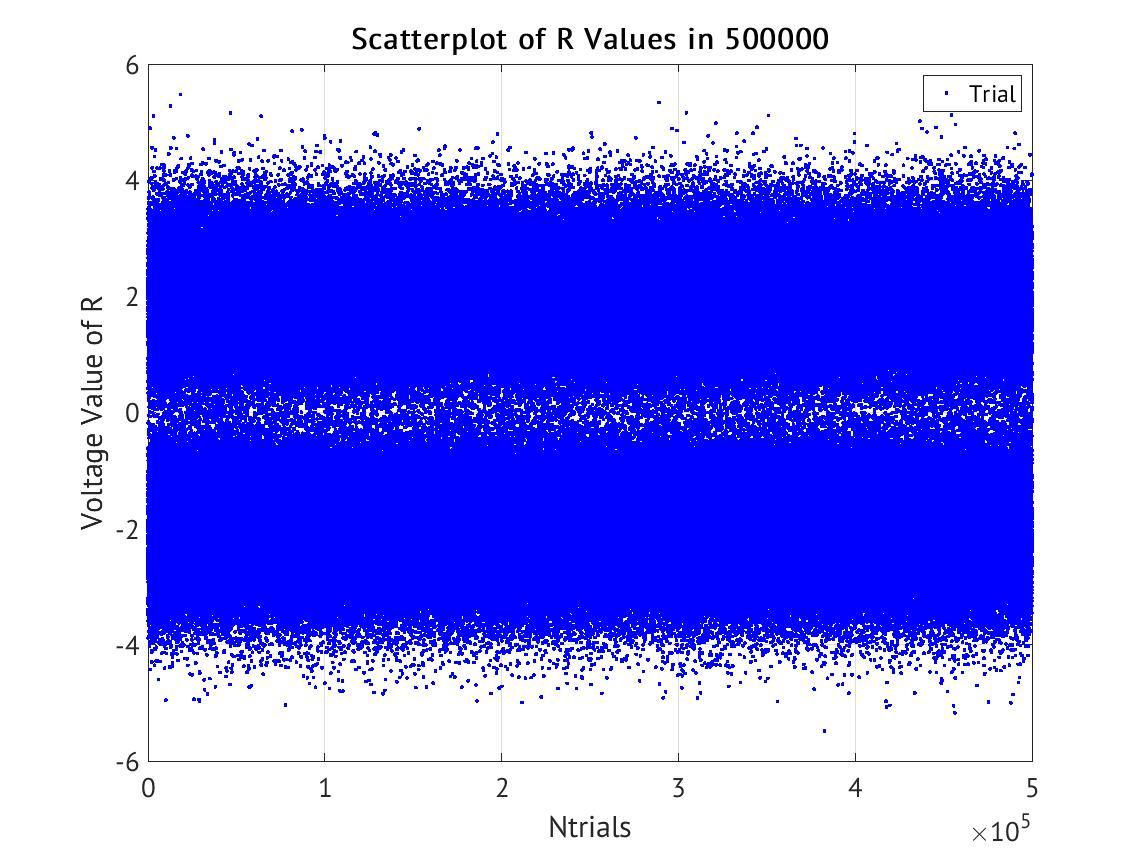
\includegraphics[width=.9\linewidth]{./Images/ScatterplotR1.jpg}
\caption{\label{fig:RScatterplot}Scatterplot of the values of R using equation 1}
\end{figure}


\noindent
Figure \ref{fig:RScatterplot} illustrates the meaning of Equation \ref{eqn:fRr} with the randomness seen around the two intended mean values \(A = \pm2\).
If the variance of the model was decreased, the plot would have much less spread from the means and be more centered around them.

\bigskip
\noindent
The histogram that represents this data is shown below here in Figure \ref{fig:RHistogram}
where the same phenomenon can be seen from both the scatterplot in Figure \ref{fig:RScatterplot} as well as from the output of Equation \ref{eqn:fRr} plotted in red on top of the histogram.
This phenomenon is illustrated as the effective probability of any value in R appearing from the trials. The values closest to the 2 means are the highest, and as you get further from them
the height decreases drastically due to the variance of the governing function.

\begin{figure}[htbp]
\centering
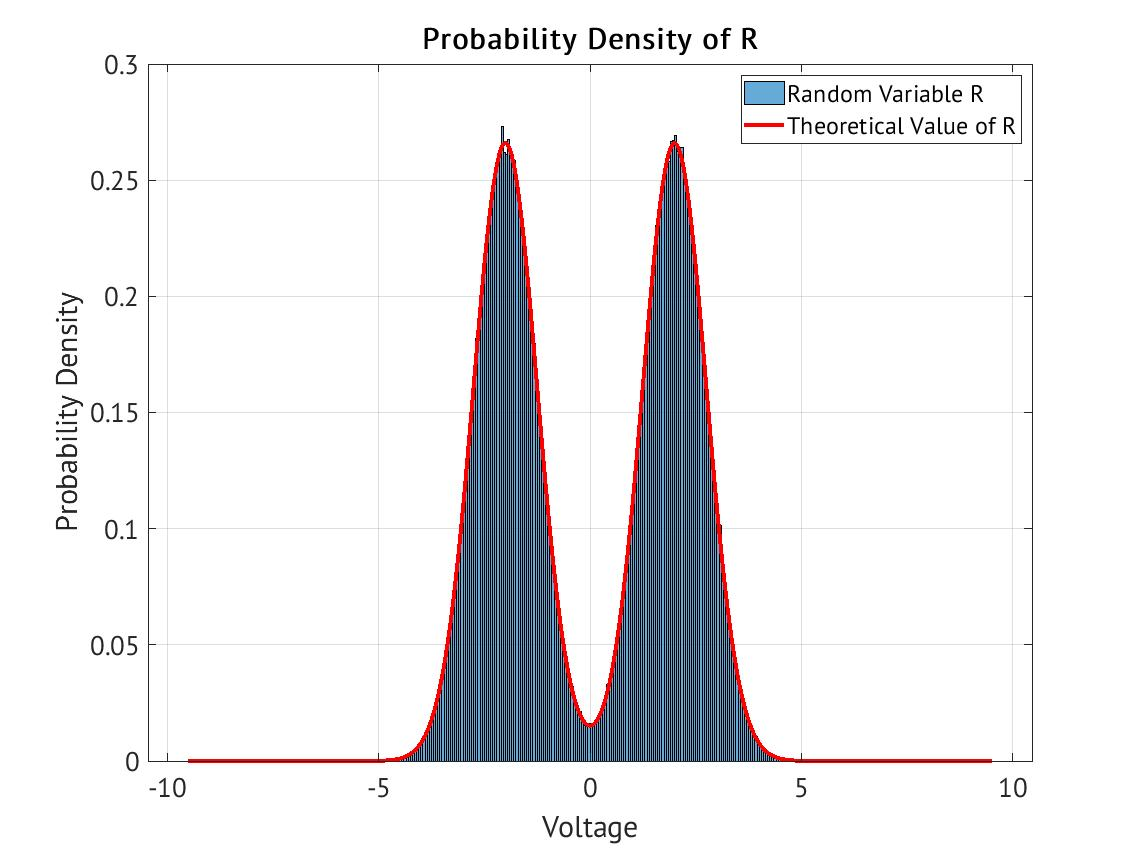
\includegraphics[width=.9\linewidth]{./Images/RPDF2.jpg}
\caption{\label{fig:RHistogram}Histogram output of the modeling of R for N = 500000 trials}
\end{figure}

\subsection{Method 1, Perfect Diode Detector}
\label{sec:org8f3b758}
\subsubsection{Analytical PDF}
\label{sec:org10c0b65}
The value of \(S\) is given by the function
\begin{equation}
\label{eqn:S1}
    S = g(R) = \begin{cases}
        \[
            0 \; \text{for} \;R < 0 \\
            R \; \text{for} \;R \geq 0
        \]
\end{equation}
\noindent
This relationship between the input variable \(R\) and the output variable \(S\) is shown below here in Figure \ref{fig:DiagramPDD}.

\begin{figure}[htbp]
\centering
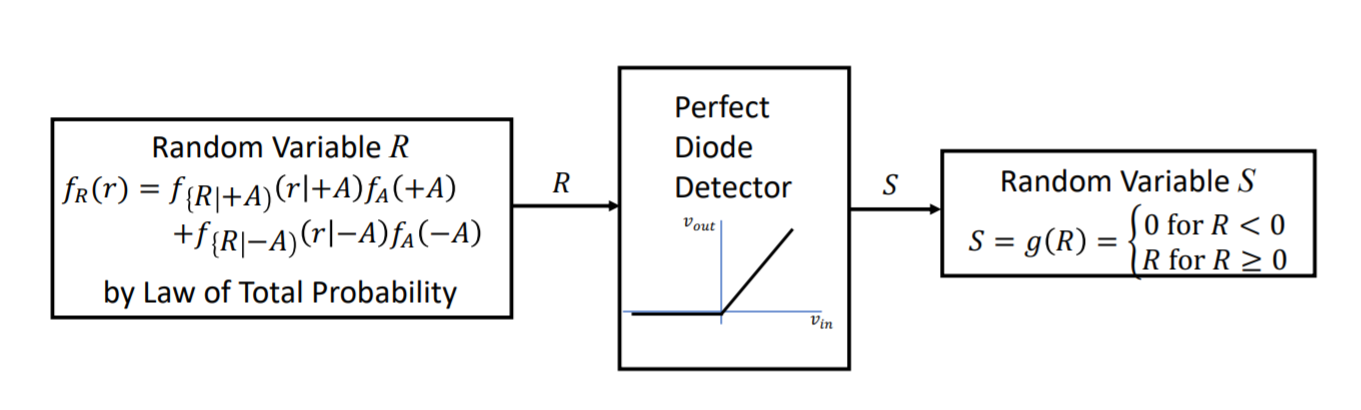
\includegraphics[width=.9\linewidth]{./Images/DiagramPDD.png}
\caption{\label{fig:DiagramPDD}Perfect Diode Detector Model for 2.2.1}
\end{figure}

\noindent
To find the function of the given random variable \(S\) the method of differentiating the CDF was used to alter the function \(f_R(r)\) into a function \(f_S(s)\).
The steps are as follows.

\noindent
The equation for \(f_R(r)\) is equivalent to
\begin{equation}
\label{eqn:fRr}
    f_R(r) = \frac{1}{2\sqrt{2\pi\sigma^2}} \left(e^{\frac{-(r-A)^2}{2\sigma^2}} + e^{\frac{-(r+A)^2}{2\sigma^2}}\right)
\end{equation}

\noindent
The value of the random variable \(S\) is defined by the above Equation \ref{eqn:S1}.
Then to find the value of \(f_S(s)\), the CDF, \(F_S(s)\) must first be found, and is derived as such

\begin{flalign}
\label{eqn:FSs}
F_S(s) & =\begin{cases} \[ 0 &s \leq 0\\ P[S \leq s] & s > 0 \end{cases}\\
     & =\begin{cases} \[ 0 &s \leq 0\\ P[R \leq s] & s > 0 \end{cases}\\
     & =\begin{cases} \[ 0 &s \leq 0\\ F_R(s) & s > 0 \end{cases}\\
     & =\begin{cases} \[ 0 &s \leq 0\\ \displaystyle \int_{-\infty}^{s} f_R(r) dr & s > 0 \end{cases}\\
\end{flalign}

\noindent
This CDF is then to be integrated, \(f_S(s) = \frac{dF_S(s)}{ds}\), to give the PDF of the function of S, \(f_S(s)\).
The result of this integration is depicted below as such

\begin{flalign*}
    f_S(s) & = \frac{d}{ds} \[ \displaystyle \int_{-\infty}^s\frac{1}{2\sqrt{2\pi\sigma^2}} \left(e^{\frac{-(r-A)^2}{2\sigma^2}} + e^{\frac{-(r+A)^2}{2\sigma^2}}\right) dr \right] \\
    & = \frac{1}{2\sqrt{2\pi\sigma^2}} \begin{bmatrix}
&\left( \displaystyle\frac{ds}{ds} \right) \times \left( e^{\frac{-(s-A)^2}{2\sigma^2}} + e^{\frac{-(s+A)^2}{2\sigma^2}} \right) \\ &- \left( \frac{d(-\infty)}{ds}\right) \times \left(  e^{\frac{-(s-A)^2}{2\sigma^2}} + e^{\frac{-(s+A)^2}{2\sigma^2}} \right) \\ &+ \displaystyle \int_{-\infty}^{s} \frac{d}{ds} \left( e^{\frac{-(s-A)^2}{2\sigma^2}} + e^{\frac{-(s+A)^2}{2\sigma^2}} \right) \end{bmatrix}  \text{for } s > 0 \\
    & = 0 \text{ for } s < 0 \\
    & = \delta(s) \times F_R(0) \text{ for } s = 0
\end{flalign*}

\noindent
With this in mind, this can thusly be simplified down into the simpler form of

\begin{equation*}
    f_S(s) = \begin{cases} \[
    0 & s < 0 \\
    F_R(0)\delta(s) & s = 0 \\
    \frac{1}{2\sqrt{2\pi\sigma^2}} \left(e^{\frac{-(s-A)^2}{2\sigma^2}} + e^{\frac{-(s+A)^2}{2\sigma^2}}\right) & s > 0 \]
\end{equation*}

\noindent
And with using the Q function to determine the value when \(s = 0\), \(F_R(0)\) is equivalent to \(\dfrac{1}{2}\delta(s)\).
Finally, with all this done, the actual analytical PDF function \(f_S(s)\) is as such

 \begin{equation}
    f_S(s) = \begin{cases} \[
    0 & s < 0 \\
    \dfrac{1}{2}\delta(s) & s = 0 \\
    \frac{1}{2\sqrt{2\pi\sigma^2}} \left(e^{\frac{-(s-A)^2}{2\sigma^2}} + e^{\frac{-(s+A)^2}{2\sigma^2}}\right) & s > 0 \]
\end{equation}

\noindent
The importance of this is due to the domain of \(R\), and how that interacts with the domain of \(S\). In this case, \(R\) has a domain of \(-\infty < R < \infty\) and \(S\) has the same domain of \(-\infty < S < \infty\).
In addition to this, the derivative of the CDF \(F_S(s)\) for each of the sections of the domain are different due to the effects of the Leibniz Rule in Appendix A.
This is what results in the \(0\) for \(s < 0\) as well as the dirac delta function when \(s = 0\).
The above PDF is shown below in Figure \ref{fig:S1Histogram} overlayed on the simulated data output.



\subsubsection{Simulated PDF}
\label{sec:org7b9bfdc}
\noindent
The relationship of the input variable \(R\) and the output variable \(S\) is shown below here in Figure \ref{fig:PerfDiodeScat} as the output voltage of the perfect diode.
The function is exactly the representation given in Figure \ref{fig:DiagramPDD}, as the output, \(S\) is zero before \(s = 0\) and becomes \(S = R\) when \(s > 0\).

\bigskip
\noindent
In Figure \ref{fig:S1Histogram}, the PDF function, as derived via the CDF method, is shown overtop of the simulated PDF. Understanding this graph is broken into three parts.
The first is the section where \(S\) is below zero, and both analytical and simulated show a value of zero. Next is the section at \(S = 0\), where there is a dirac delta function with an area of \(0.5\).
This is due to the section of the domain of \(R\) that is below \(0\) is now put entirely into the bin for \(0\), effectively putting half of the outputs into this bin and creating the dirac delta function.
Thirdly is the area where the curve is maintained from that of Figure \ref{fig:RHistogram}, with the same values within each of the bins.

\begin{figure}[htbp]
\centering
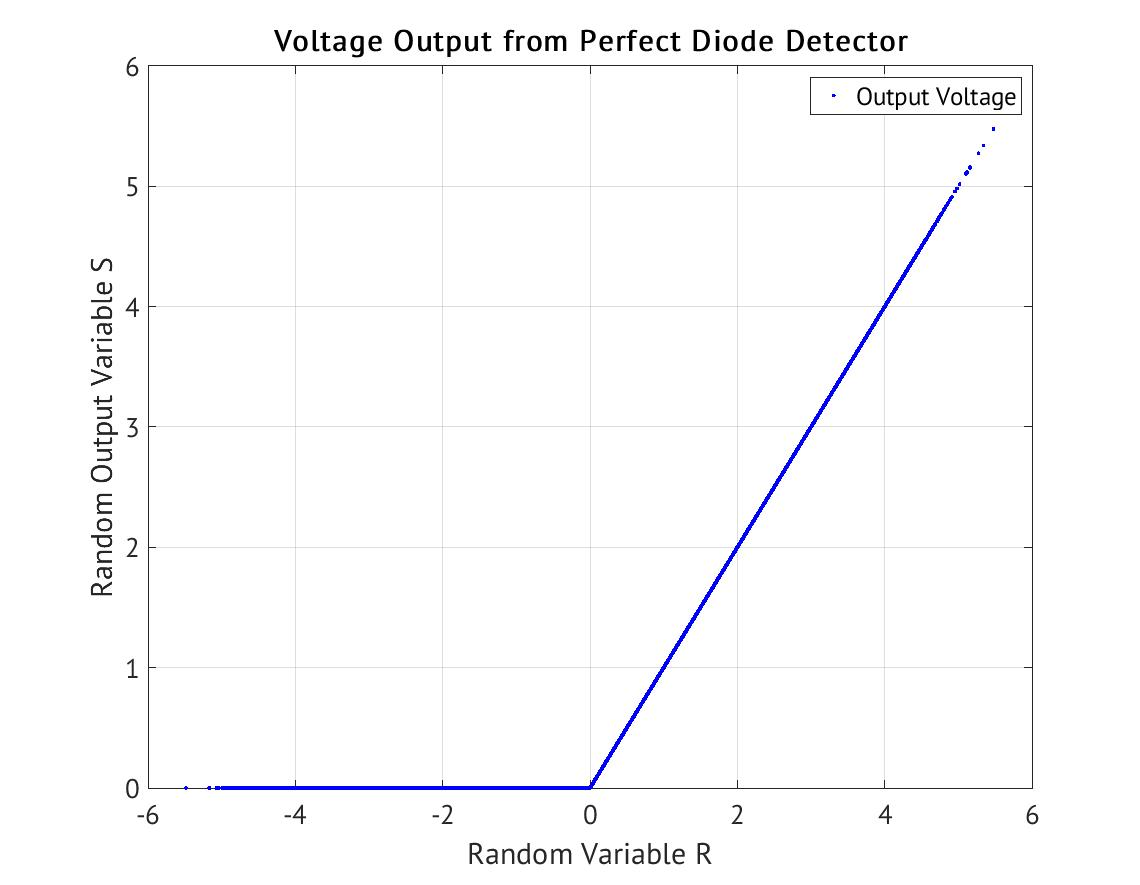
\includegraphics[width=.9\linewidth]{./Images/PerfDiode3.jpg}
\caption{\label{fig:PerfDiodeScat}Relationship of Random Variables R and S in terms of the Perfect Diode Detector Function}
\end{figure}

\begin{figure}[htbp]
\centering
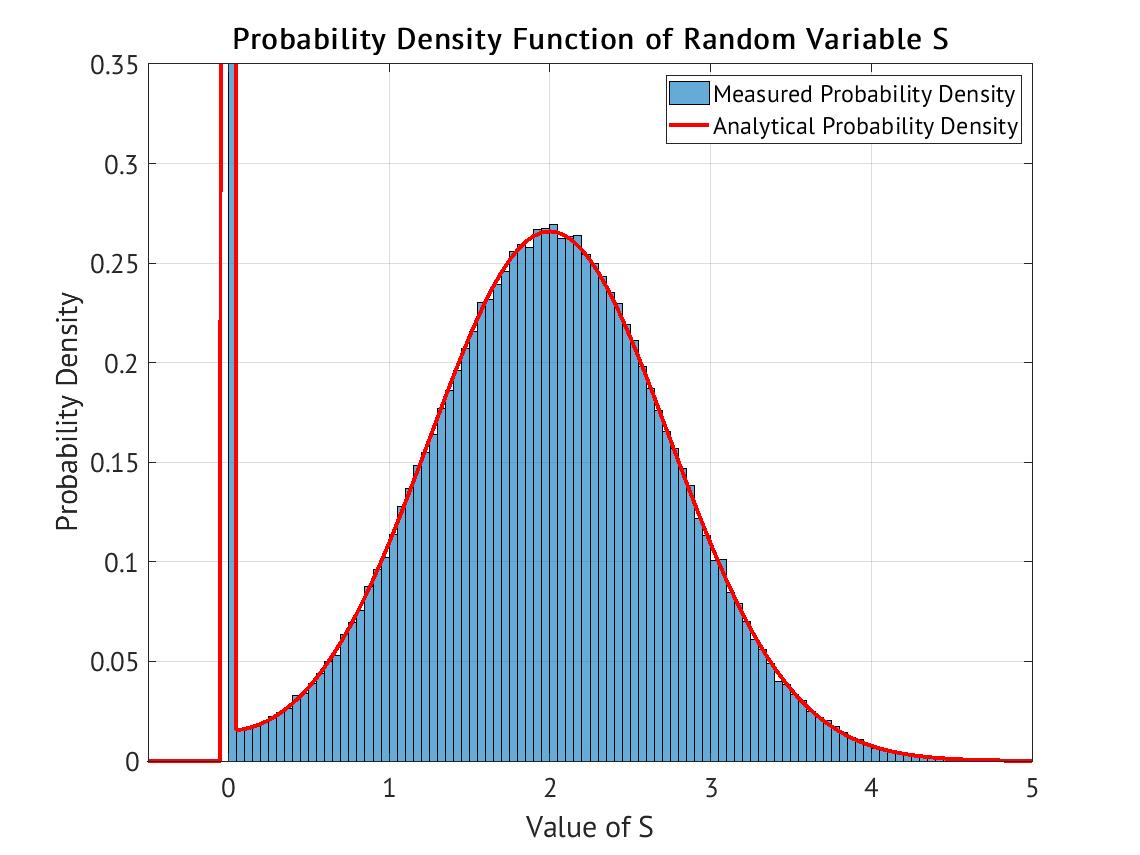
\includegraphics[width=.9\linewidth]{./Images/S1PDF4.jpg}
\caption{\label{fig:S1Histogram}Analytical and Simulated PDF functions of the given function of the random variable S}
\end{figure}

\smallskip
\bigskip
\noindent
Lastly, the expected value of \(S\) is calculated as \(1.0010\), which in context of the function, makes sense given the majority of the distribution is between \(0\) and \(2\).
In addition to this, the value of \(g(E[R])\) is calculated to be about \(0.0022\). These will be referenced again, in section \ref{sec:orged66029}.

\subsection{Method 2, Absolute Value Detector}
\label{sec:org6b004cd}
\subsubsection{Analytical PDF}
\label{sec:org0f2b302}
In this case, the value of \(S\) is determined by the function shown below in Figure \ref{fig:S2Diagram}.

\begin{figure}[htbp]
\centering
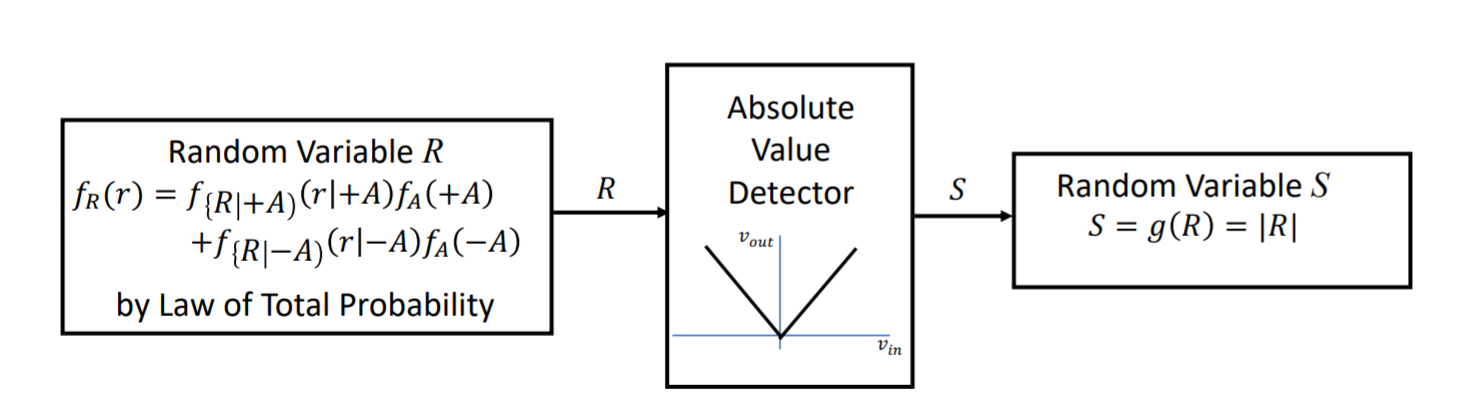
\includegraphics[width=.9\linewidth]{./Images/S2Diagram.png}
\caption{\label{fig:S2Diagram}Absolute Value Detector model for 2.3.1}
\end{figure}

\noindent
To find the function of the random variable \(S\) is different than that of Method 1 above in 2.2.1. The function for \(S\) of given random variable \(R\) is \(S = g(R) = |R|\). The method for finding this PDF is as such

\begin{equation}
\label{eqn:analyticalPDF}
    f_S(s) = \left[ \frac{1}{|ds / dr|} f_R(r) \right]_{r = g^{-1}(s)}
\end{equation}

\bigskip
\noindent
Breaking this into parts for solving leads to the following

\begin{equation}
\label{eqn:gFunc1}
    \begin{gathered}
        S = g(R) = |r| \\
        R = g^{-1}(S) = \pm s \\
    \end{gathered}
\end{equation}

\begin{equation}
\label{eqn:PSis0}
    f_S(0) = P[S = 0] = 2P[R = 0] \rightarrow P[R = 0] = 0.0154 \times 2 = 0.0308
\end{equation}

\noindent
The value for \(s = 0\) is the above Equation \ref{eqn:PSis0}, which is defined as the value of Equation \ref{eqn:fRr} at the value of \(r = 0\), which is the number \(0.0154\).
This is then multiplied by a factor of 2 given that the function of \(S\) has a domain of \(s \geq 0\), effectively mapping the positive and negative values very near \(0\) in \(R\) to \(0\) in \(S\).
Thus, \(0.0154 \times 2 = 0.0308\).

\begin{equation}
\label{eqn:dsOverdr}
    \begin{gathered}
        \frac{ds}{dr} = \frac{s}{|s|} \\
        \left| \frac{ds}{dr} \right| = \left| \frac{s}{|s|} \right| \rightarrow 1
    \end{gathered}
\end{equation}

\bigskip
\noindent
These (\ref{eqn:gFunc1}, \ref{eqn:PSis0}, \ref{eqn:dsOverdr}) can then be substituted into Equation \ref{eqn:analyticalPDF} as such

\begin{equation}
\label{eqn:analyticalMethod}
    f_S(s) = \left[ \frac{1}{1} f_R(r) \right]_{r = \pm s} \rightarrow  f_R(+s) - f_R(-s)  \rightarrow f_R(s) + f_R(s) \rightarrow 2f_R(s)
\end{equation}

\bigskip
\noindent
Which then leads to the analytical PDF function for all values of \(R\)

\begin{equation}
\label{eqn:fS2s}
    f_S(s) = \begin{cases} \[
    0 & s < 0 \\
    0.0308 & s = 0 \\
    \frac{1}{\sqrt{2\pi\sigma^2}} \left(e^{\frac{-(s-A)^2}{2\sigma^2}} + e^{\frac{-(s+A)^2}{2\sigma^2}}\right) & s > 0 \]
\end{equation}

\bigskip
\noindent
The output of this defined function is shown below in Figure \ref{fig:S2PDF}. Along with this data is the simulated data obtained.

\subsubsection{Simulated PDF}
\label{sec:org55d1300}
With the function of \(g(R)\) defined, running the trials for \(S\) results in the scatterplot shown here in Figure \ref{fig:S2Scat}.

\begin{figure}[htbp]
\centering
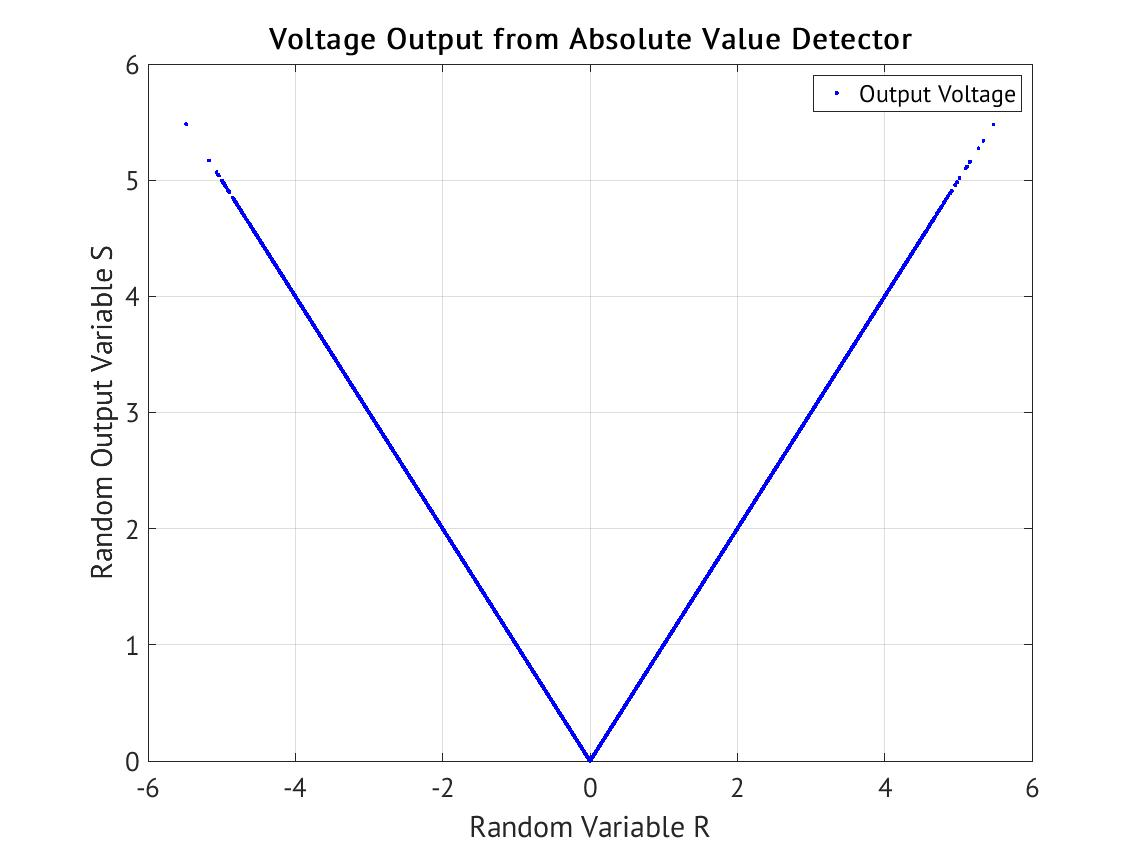
\includegraphics[width=.9\linewidth]{./Images/AbsVal5.jpg}
\caption{\label{fig:S2Scat}Scatterplot results of Absolute Value Detector model on random Variable R}
\end{figure}

\bigskip
\noindent
Figure \ref{fig:S2Scat} shows that the output of the function is in fact the random variable \(S\) as it is defined above in Figure \ref{fig:S2Diagram}.
The histogram of this same dataset is shown in Figure \ref{fig:S2PDF}, with the analytical function (Equation \ref{eqn:fS2s}) as derived in 2.3.1.

\begin{figure}[htbp]
\centering
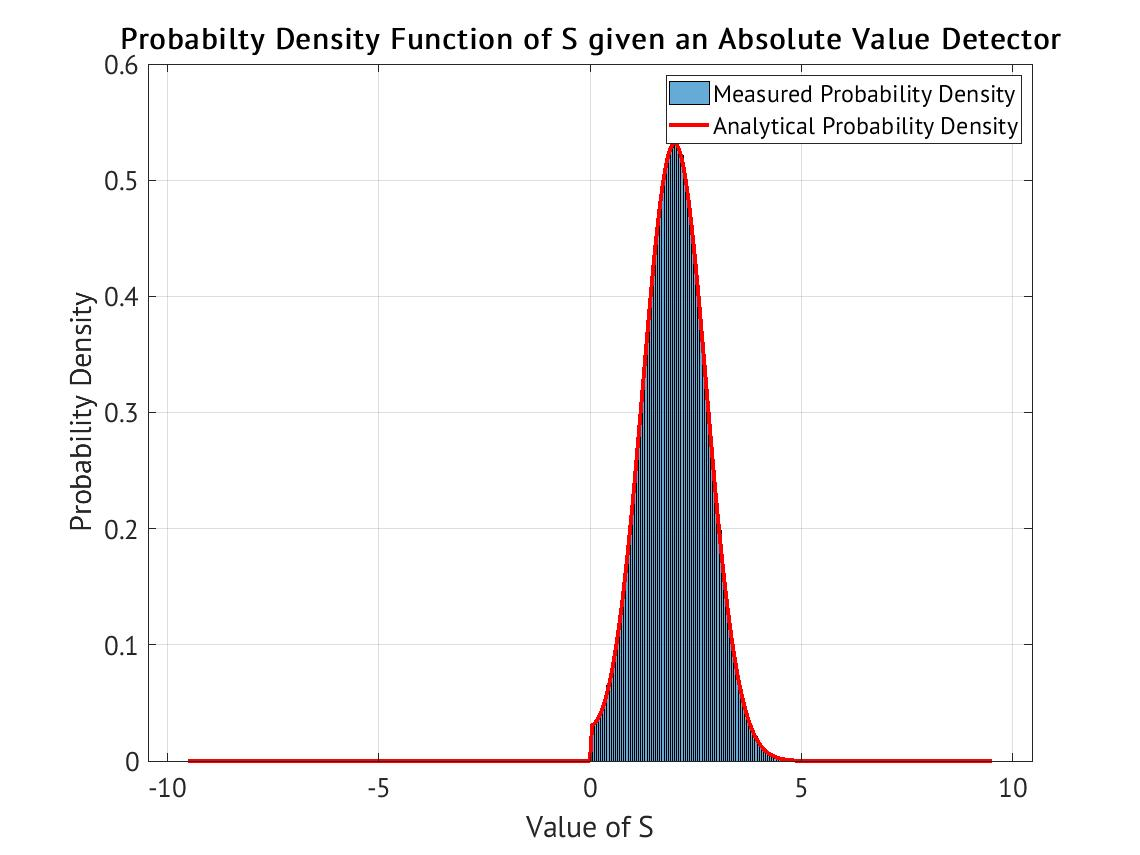
\includegraphics[width=.9\linewidth]{./Images/S2PDF6.jpg}
\caption{\label{fig:S2PDF}Analytical and Simulated PDF functions of the derived function of the random Variable S}
\end{figure}

\bigskip
\noindent
Analyzing this data shows that the relative densities of each of the bins is just about double what the same bins were in Figure \ref{fig:S1Histogram}, and is expected due to how the absolute value of a variable functions.
Both the analytical and the simulated are just on track for what is expected and represent the data in the correct manner.

\bigskip
\noindent
In addition to this information, the expected value of \(S\) is found within the simulation to be around \(1.9997\) and the expected value of \(g(R)\) is found to be \(0.0022\).
The expected value of \(S\) is entirely expected as there is only a single ``hump'' in this output function, which has a mean of \(2\) based on how it is defined.
Both of these values will be examined further in \ref{sec:orged66029}.

\subsection{Method 3, Square Law Detector}
\label{sec:org2e1d02d}
\subsubsection{Analytical PDF}
\label{sec:org92a4c94}
The value of \(S\) is given by the function

\begin{equation}
\label{eqn:S3}
    S = g(R) = R^2
\end{equation}

\bigskip
\noindent
This relationship between the input variable \(R\) and the output variable \(S\) below in Figure \ref{fig:DiagramSLD}.

\begin{figure}[htbp]
\centering
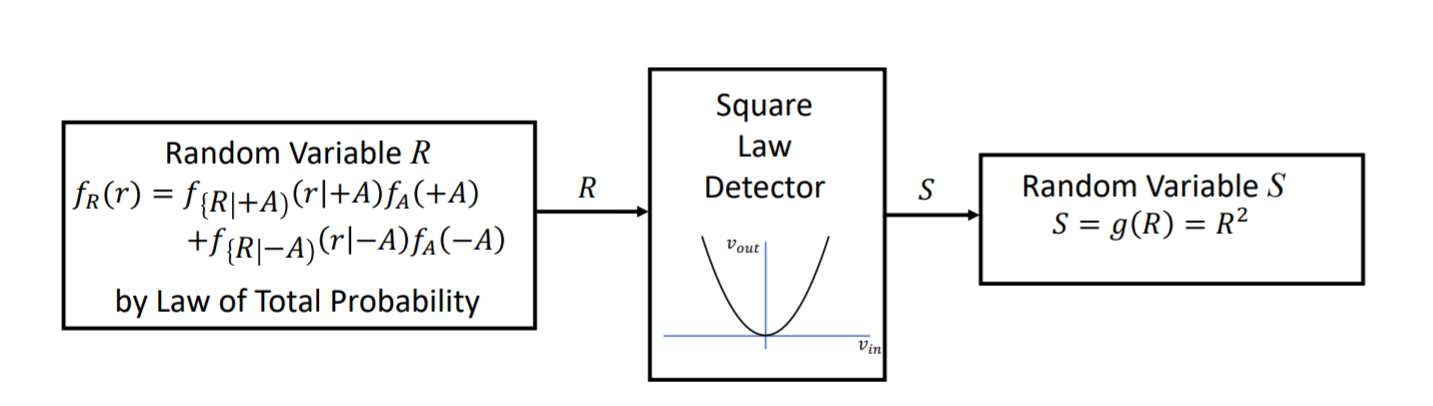
\includegraphics[width=.9\linewidth]{./Images/DiagramSLD.png}
\caption{\label{fig:DiagramSLD}Square Law Detector model for 2.4.1}
\end{figure}

\noindent
Similarly to Section \ref{sec:org8f3b758}, the CDF method was used to find the analytical PDF of the described function. This process is documented below.

\bigskip
\noindent
The function of \(R\) is the same as before in Equation \ref{eqn:fRr}, shown again here below.

\begin{equation*}
    f_R(r) = \frac{1}{2\sqrt{2\pi\sigma^2}} \left(e^{\frac{-(r-A)^2}{2\sigma^2}} + e^{\frac{-(r+A)^2}{2\sigma^2}}\right)
\end{equation*}

\bigskip
\noindent
The value of \(S\) given this function is derived in a similar manner as was done above in \ref{sec:org8f3b758}, starting with the definition of \(F_S(s)\) in Equation \ref{eqn:FSs}.
Restating this definition is as such

\begin{flalign*}
F_S(s) & =\begin{cases} \[ 0 &s \leq 0\\ P[S \leq s] & s > 0 \end{cases}\\
     & =\begin{cases} \[ 0 &s \leq 0\\ P[R \leq s] & s > 0 \end{cases}\\
     & =\begin{cases} \[ 0 &s \leq 0\\ F_R(s) & s > 0 \end{cases}\\
     & =\begin{cases} \[ 0 &s \leq 0\\ \displaystyle \int_{-\infty}^{\sqrt{s}} f_R(r) dr & s > 0 \end{cases}\\
\end{flalign*}

\noindent
This then leads to the PDF function as the derivative of this is taken. The methodology of this is once again, very similar to that used in Method 1. The derivative is shown here below.

\begin{flalign*}
    f_S(s) & = \frac{d}{ds} \[ \displaystyle \int_{-\infty}^{\sqrt{s}}\frac{1}{2\sqrt{2\pi\sigma^2}} \left(e^{\frac{-(r-A)^2}{2\sigma^2}} + e^{\frac{-(r+A)^2}{2\sigma^2}}\right) dr \right] \\
    & = \frac{1}{2\sqrt{2\pi\sigma^2}} \begin{bmatrix}
&\left( \displaystyle\frac{d\sqrt{s}}{ds} \right) \times \left( e^{\frac{-(\sqrt{s}-A)^2}{2\sigma^2}} + e^{\frac{-(\sqrt{s}+A)^2}{2\sigma^2}} \right) \\ &- \left( \frac{d(-\infty)}{ds}\right) \times \left(  e^{\frac{-(\sqrt{s}-A)^2}{2\sigma^2}} + e^{\frac{-(\sqrt{s}+A)^2}{2\sigma^2}} \right) \\ &+ \displaystyle \int_{-\infty}^{\sqrt{s}} \frac{d}{ds} \left( e^{\frac{-(\sqrt{s}-A)^2}{2\sigma^2}} + e^{\frac{-(\sqrt{s}+A)^2}{2\sigma^2}} \right) \end{bmatrix}  \text{for } s \geq 0 \\
    & = 0 \text{ for } s < 0 \\
\end{flalign*}

\noindent
When this is simplified down it yields the equation as follows.

\begin{equation}
\label{eqn:fS3s}
    f_S(s) = \begin{cases} \[
    0 & s < 0 \\
    \frac{1}{2\sqrt{2\pi\sigma^2}} \left(e^{\frac{-(s-A)^2}{2\sigma^2}} + e^{\frac{-(s+A)^2}{2\sigma^2}}\right) & s \geq 0 \]
\end{equation}

\bigskip
\noindent
There is a step in this process similar to what is used in Equation \ref{eqn:analyticalMethod}, where the inverse function of both the absolute value, as well as the square of \(R\), end up having both a positive and negative component. This is then resolved by subtracting the negative from the positive, which is the same as just doubling the function itself. This is what gives the final equation \ref{eqn:fS3s}.


\bigskip
\noindent
This is displayed below in Figure \ref{fig:S3PDF}, where this analytical function is overlayed on top of the simulated histogram.

\subsubsection{Simulated PDF}
\label{sec:org1359bfc}
The defined function of \(S\) is defined above in Figure \ref{fig:DiagramSLD}, and when the simulated trials are run, the output scatterplot of the results is shown in Figure \ref{fig:S3Scat}.

\begin{figure}[htbp]
\centering
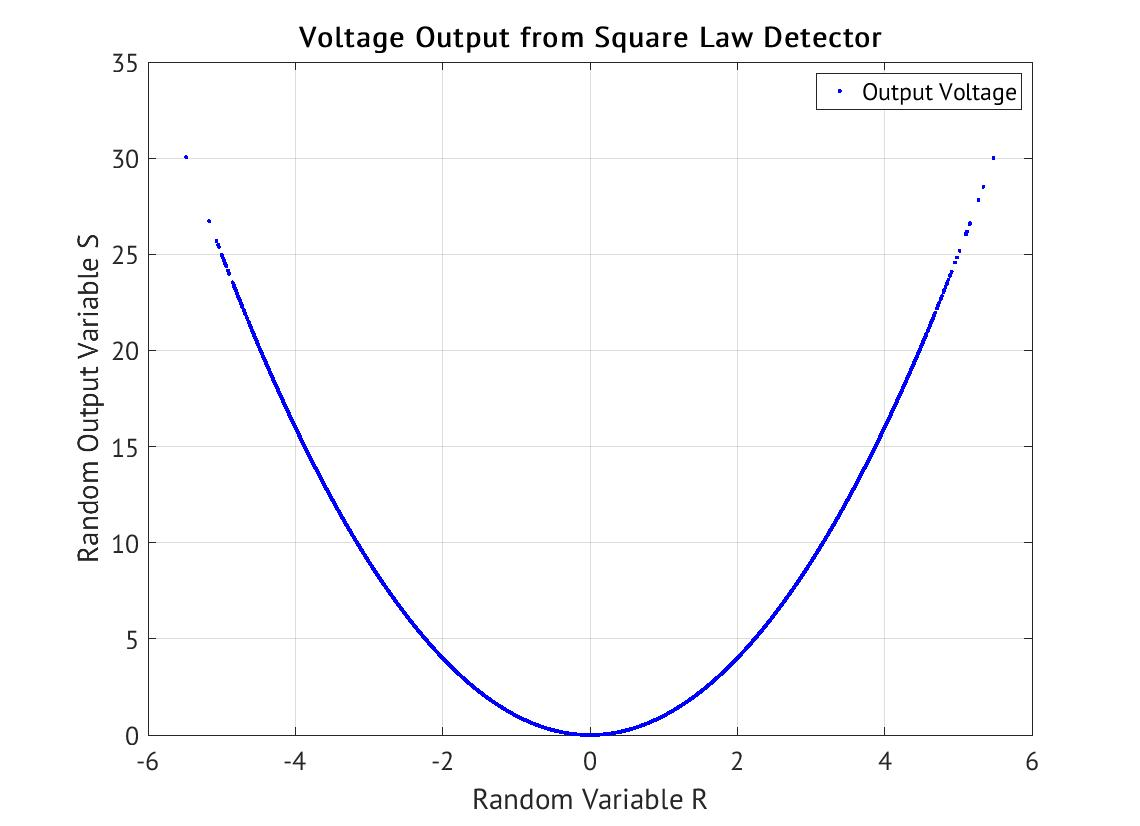
\includegraphics[width=.9\linewidth]{./Images/SquareLaw7.jpg}
\caption{\label{fig:S3Scat}Scatterplot results of Square Law Detector model on random variable R}
\end{figure}


\noindent
This scatterplot is the expected output of the function \(S\) given \(R\). This is then complemented by the corresponding histogram, Figure \ref{fig:S3PDF}, below.

\begin{figure}[htbp]
\centering
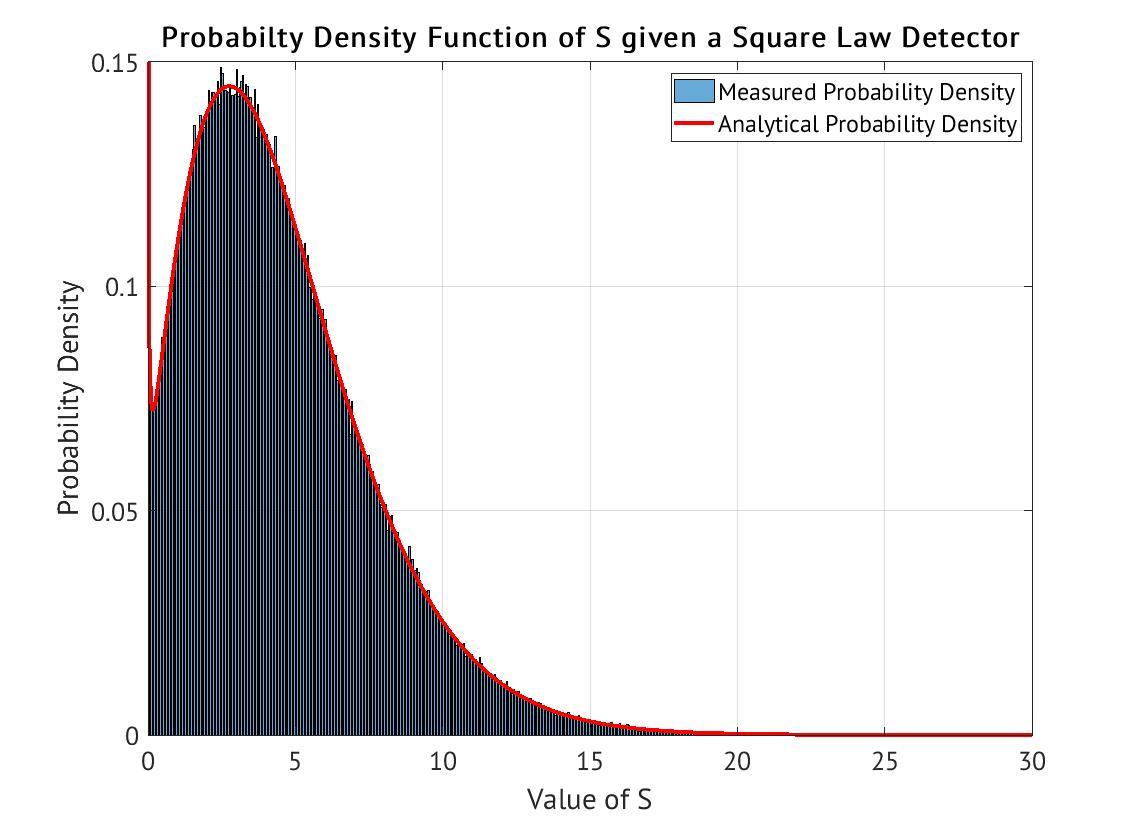
\includegraphics[width=.9\linewidth]{./Images/S3PDF8.jpg}
\caption{\label{fig:S3PDF}Analytical and Simulated PDF functions of derived function of random variable S}
\end{figure}

\bigskip
\noindent
The output of this function in not instantly understandable upon initial inspection.
Taking a deeper look into this shows both the simulated and analytical functions having a large spike at \(S = 0\), this is due to how squaring very small numbers work.
If a number less than \(1\) is squared, the value that is obtained is going to be less than the input value. This effect is much more prominent as the input gets closer to \(0\).
So, if there is a value between \(0\) and \(1\), that is pushed closer and closer to the corresponding bin.
That is why as the function gets nearer and nearer to \(0\) the probability density goes to \(\infty\).

\bigskip
\noindent
Moving past the values near zero, the peak is somewhere around \(4\), which is exactly the square of the input means \(2\) and \(-2\). The long tapering of the function towards a much larger \(S\) value compared to the previous functions is due to how larger numbers grow much faster when squared as compared to smaller numbers. Thus, the density of a larger number (in either positive or negative direction) is much lower than that of many nearer to that of the square of the means, but any outliers are pushed further and further away from said value.

\bigskip
\noindent
The measured mean from the simulation is found to be around \(4.5529\), just above the square of (either) of the means. The expected value of \(g(R)\) is then found as well to be very very small, nearly \(0\).


\subsection{Jensen's Inequality}
\label{sec:orged66029}
The values of the expectation of the random variables \(S\), as well as the expected values of the functions of \(R\), \(g(R)\) are captured below in Table \ref{tab:ExpectedVals}.

\begin{table}[htbp]
\caption{\label{tab:ExpectedVals}Expected values of both random variable S and respective function of R}
\centering
\begin{tabular}{|c|c|c|c|}
\hline
Method & Function of R & E[S] & E[g(R)]\\
\hline
1 & R, R \(\ge\) 0 & 1.0010 & 0.0022\\
2 & \lvert R \rvert & 1.9997 & 0.0022\\
3 & R\textsuperscript{2} & 4.5529 & 0.0000\\
\hline
\end{tabular}
\end{table}

\bigskip
\noindent
As can be seen from Table \ref{tab:ExpectedVals}, the expected values of each version of \(S\) is always greater than the expected values of the corresponding \(g(R)\). This is equivalent to saying that the expected value of \(g(R)\) is always less than or equal to that of the expected value of \(S\).
This is what Jensen's Inequality is. The data specifically shows the phenomenon happening, and showing what is exactly expected.

\section{What was Learned}
\label{sec:org25fcc23}
This project consisted of multiple random variables, and the interaction of different functions on a random variable (consisting of different random variables) to get different outputs. These were then parsed and implemented into code in 2 major ways.

\bigskip
\noindent
The major methods of understanding the concepts of this project were through simulation of random variables and data, as well as deriving and explaining the analytical functions that describe the phenomena represented through the histograms. The use of actual Calculus and other different parts of math was engaging and informative during the process of understanding the project and its goals for what was to be learned.
Overall, I feel that this project has helped me better understand the concepts, and forces me to seriously understand what I am doing to not only create, but to then explain the outputs of the code produced.


\subsection{Issues and Changes}
\label{sec:org3a967bc}
There were minimal issues with the content of the project as a whole. Personally, I feel that there was just some confusion that came from the inclusion of the skeleton code with conflicting information and directions to that of the project document.
If this issue were to have been avoided, there would have been many less perceived problems in this. Other than that, this project was not specifically hard in terms of content, but did require a specific understanding of both what is going on in lectures, as well as how to explain them back in a meaningful sense.

\bigskip
\noindent
From doing this project, I do not believe that any major changes are really needed. If there is to be a skeleton code that is included the next time that this is used, I believe that that would have to be ironed out first. On top of this, the report format of having the analytical section before the simulated in all three cases is a bit jarring for myself, as the information that is easiest to digest should be first (in my opinion). That would be the figures for the simulated sections, then the math behind how the graphs (that would have already been seen by that point) were made with the derivations in the analytical section.

\bigskip
\noindent
The amount of time spent on this project is a bit variable. Because of the confusion that I had personally before 3/14/22, there was some amount of time and energy wasted as I had misunderstood what was being asked of myself for this project. After that date there were many things that were cleared up and allowed myself to focus on what the project was asking for sure this time.
If the time is to be measured from the very beginning, I would estimate the time spent to be around 20 hours total. After the information from the 14th, I would say the non wasted energy and time would end up being around 16 hours.
\end{document}
